\section{Exercises from the French baccalaureate}
%<-------------------------------------------------------------------------->
Graph theory was taught in the last year of the French \emph{lycée}
(option \emph{mathématiques} of the \emph{série ES}). Here are exercises given
at the \emph{baccalauréat} between 2003 and 2006, translated into English. All
the graphs are drawn with \tkzname{tkz-graph}; the code of each graph follows
the exercise.

%<-------------------------------------------------------------------------->
\subsection{North America, June 2003}\label{an03}
%<-------------------------------------------------------------------------->
Let $G$ be the graph below, with the vertices A, B, C, D, E, F and G.

\begin{enumerate}
\item What is its order? What is the degree of each vertex?
\item Copy and complete the table of the distances between two vertices of
      $G$:

\medskip
\begin{center}
\begin{tabular}{|l|c|c|c|c|c|c|c|}\hline
Distance & A & B & C & D & E & F & G \\ \hline
A        & X &   &   &   &   &   &   \\ \hline
B        & X & X &   &   &   &   &   \\ \hline
C        & X & X & X &   &   &   &   \\ \hline
D        & X & X & X & X &   &   &   \\ \hline
E        & X & X & X & X & X &   &   \\ \hline
F        & X & X & X & X & X & X &   \\ \hline
G        & X & X & X & X & X & X & X \\ \hline
\end{tabular}
\end{center}

\medskip
Deduce the diameter of this graph.
\item
   \begin{enumerate}
   \item Give a complete subgraph of order 3 of $G$. What can you deduce for
         the chromatic number of $G$?
   \item Propose a coloring of $G$ and deduce its chromatic number.
   \end{enumerate}
\item Give the matrix $M$ of $G$ (rows and columns in alphabetical order).
\item Using the matrix $M^2$ below, find the number of chains of length 2
      starting from A and not returning to A.
\end{enumerate}

\medskip
\begin{minipage}{9cm}
\begin{tikzpicture}[scale=.9]
  \Vertex[x=1.3,y=3.8]{A}  \Vertex[x=4.2,y=5.5]{B}
  \Vertex[x=7.3,y=4]{C}    \Vertex[x=8.5,y=1.5]{D}
  \Vertex[x=5,y=0]{E}      \Vertex[x=3.6,y=4]{F}
  \Vertex[x=0.7,y=1]{G}
  \Edges(A,B,C,D,E,G,A,F,E,C) \Edge(B)(F)
\end{tikzpicture}
\end{minipage}
\hfill
\begin{minipage}{6cm}
$M^2 =
\begin{pmatrix}
3 & 1 & 1 & 0 & 2 & 1 & 0\\
1 & 3 & 0 & 1 & 2 & 1 & 1\\
1 & 0 & 3 & 1 & 1 & 2 & 1\\
0 & 1 & 1 & 2 & 1 & 1 & 1\\
2 & 2 & 1 & 1 & 4 & 0 & 0\\
1 & 1 & 2 & 1 & 0 & 3 & 2\\
0 & 1 & 1 & 1 & 0 & 2 & 2
\end{pmatrix}$
\end{minipage}

\medskip
The answer to question 4 is given by \tkzcname{tkzAdjacencyMatrix}, used just
after the picture: $M = \tkzAdjacencyMatrix$

\begin{tkzexample}[code only]
\begin{tikzpicture}
  \Vertex[x=1.3,y=3.8]{A}  \Vertex[x=4.2,y=5.5]{B}
  \Vertex[x=7.3,y=4]{C}    \Vertex[x=8.5,y=1.5]{D}
  \Vertex[x=5,y=0]{E}      \Vertex[x=3.6,y=4]{F}
  \Vertex[x=0.7,y=1]{G}
  \Edges(A,B,C,D,E,G,A,F,E,C) \Edge(B)(F)
\end{tikzpicture}
$M = \tkzAdjacencyMatrix$
\end{tkzexample}

\newpage
%<-------------------------------------------------------------------------->
\subsection{French West Indies and Guiana, June 2003}\label{ag03}
%<-------------------------------------------------------------------------->
\begin{enumerate}
\item A museum has 9 rooms, named A, B, C, D, E, F, G, H and S. Here is the
      plan of the museum:

\medskip
\begin{center}
\begin{tikzpicture}[scale=.8]
  \draw (0,0) rectangle (8,6);
  \foreach \x in {2,4,6}{%
    \draw (\x,0)--(\x,0.7)   (\x,1.3)--(\x,2.7)
          (\x,3.3)--(\x,4.7) (\x,5.3)--(\x,6);}
  \draw (2,2)--(2.7,2) (3.3,2)--(4.7,2) (5.3,2)--(6,2);
  \draw (2,4)--(2.7,4) (3.3,4)--(4.7,4) (5.3,4)--(8,4);
  \foreach \r/\p in {S/{1,3},G/{3,3},D/{3,1},A/{3,5},H/{5,1},
                     E/{5,3},B/{5,5},F/{7,2},C/{7,5}}
    \node at (\p) {\r};
\end{tikzpicture}
\end{center}

\medskip
A visitor in the room S can go directly to the rooms A, B or G. From the
room C, he can go directly to the room B but not to the room F. We study
the walk of a visitor in the museum, without caring about how he enters or
leaves it. The situation is modeled by a graph: the vertices are the rooms
and the edges are the doors.

   \begin{enumerate}
   \item Draw a graph modeling this situation.
   \item Is it possible to visit the museum using each door once and only
         once? Justify with a theorem of the course.
   \item The curator wants each room to have a carpet different from the
         carpets of the neighboring rooms (rooms joined by a door). What is
         the minimum number of kinds of carpet? Justify.
   \end{enumerate}
\item Let $M$ be the $9\times 9$ matrix of this graph, the rooms being in the
      order S, A, B, C, D, E, F, G, H. The graph is not directed: what is the
      consequence for the matrix?
\item Here is the matrix
\[M^4 =
\begin{pmatrix}
18 & 12 & 11 & 2 & 20 & 12 & 6 & 12 & 12\\
12 & 20 & 3 & 6 & 11 & 20 & 5 & 18 & 5\\
11 & 3 & 16 & 0 & 19 & 3 & 8 & 4 & 12\\
2 & 6 & 0 & 3 & 1 & 7 & 1 & 4 & 1\\
20 & 11 & 19 & 1 & 31 & 9 & 11 & 12 & 19\\
12 & 20 & 3 & 7 & 9 & 28 & 9 & 20 & 9\\
6 & 5 & 8 & 1 & 11 & 9 & 9 & 8 & 9\\
12 & 18 & 4 & 4 & 12 & 20 & 8 & 20 & 6\\
12 & 5 & 12 & 1 & 19 & 9 & 9 & 6 & 17
\end{pmatrix}\]
   \begin{enumerate}
   \item How many paths of 4 steps start from D and come back to D?
   \item How many paths of 4 steps start from S and end in C? Give them.
   \item Is it always possible to join two rooms in 4 steps? Justify.
   \end{enumerate}
\end{enumerate}

\newpage
The plan is drawn with \TIKZ\ only:

\begin{tkzexample}[code only]
\begin{tikzpicture}
  \draw (0,0) rectangle (8,6);
  \foreach \x in {2,4,6}{%
    \draw (\x,0)--(\x,0.7)   (\x,1.3)--(\x,2.7)
          (\x,3.3)--(\x,4.7) (\x,5.3)--(\x,6);}
  \draw (2,2)--(2.7,2) (3.3,2)--(4.7,2) (5.3,2)--(6,2);
  \draw (2,4)--(2.7,4) (3.3,4)--(4.7,4) (5.3,4)--(8,4);
  \foreach \r/\p in {S/{1,3},G/{3,3},D/{3,1},A/{3,5},H/{5,1},
                     E/{5,3},B/{5,5},F/{7,2},C/{7,5}}
    \node at (\p) {\r};
\end{tikzpicture}
\end{tkzexample}

\newpage
%<-------------------------------------------------------------------------->
\subsection{Asia, June 2003}\label{asj03}
%<-------------------------------------------------------------------------->
\begin{minipage}[t]{0.58\textwidth}
In the town of GRAPH, we study the main streets joining the places open to
the public: the town hall (M), the shopping center (C), the library (B), the
swimming pool (P) and the high school (L). The table gives the streets
between these places.
\end{minipage}\hfill
\begin{minipage}[t]{0.38\textwidth}
\begin{center}
\begin{tabular}{|*{5}{c|} c|} \cline{2-6}
\multicolumn{1}{c|}{} & B & C & L & M & P \\ \hline
B &   & X &   & X & X \\ \hline
C & X &   & X & X &   \\ \hline
L &   & X &   & X &   \\ \hline
M & X & X & X &   & X \\ \hline
P & X &   &   & X &   \\ \hline
\end{tabular}
\end{center}
\end{minipage}

\begin{enumerate}
\item Draw a graph representing this situation.
\item Show that there is a route using each street of this plan once and
      only once. Justify and propose such a route.

      Is there such a route starting and ending at the same place?
\item Dimitri lives in this town. The graph below gives the \textbf{new}
      plan of the district, with the directions of traffic in the streets and
      the travel times between the places (D is the home of Dimitri).
\end{enumerate}

\begin{center}
\begin{tikzpicture}
  \SetGraphUnit{3}
  \tkzSetUpGraph[light fill=gray!40,label fill=white]
  \Vertex{P}
  \NOEA(P){B} \SOEA(P){M} \NOEA(B){D}
  \SOEA(B){C} \SOEA(C){L}
  \Edge[<->,label=$4$](P)(M)
  \Edge[<->,label=$9$](C)(M)
  \Edge[<->,label=$4$](C)(L)
  \Edge[<->,label=$5$](C)(D)
  \Edge[<->,label=$10$](B)(M)
  \Edge[<->,label=$11$,style={bend right}](L)(D)
  \Edge[->,label=$3$](C)(B)
  \Edge[->,label=$10$](D)(B)
  \Edge[->,label=$10$](L)(M)
  \Edge[->,label=$10$](B)(P)
\end{tikzpicture}
\end{center}

\newpage
\begin{tkzexample}[code only]
\begin{tikzpicture}
  \SetGraphUnit{3}
  \tkzSetUpGraph[light fill=gray!40,label fill=white]
  \Vertex{P}
  \NOEA(P){B} \SOEA(P){M} \NOEA(B){D}
  \SOEA(B){C} \SOEA(C){L}
  \Edge[<->,label=$4$](P)(M)
  \Edge[<->,label=$9$](C)(M)
  \Edge[<->,label=$4$](C)(L)
  \Edge[<->,label=$5$](C)(D)
  \Edge[<->,label=$10$](B)(M)
  \Edge[<->,label=$11$,style={bend right}](L)(D)
  \Edge[->,label=$3$](C)(B)
  \Edge[->,label=$10$](D)(B)
  \Edge[->,label=$10$](L)(M)
  \Edge[->,label=$10$](B)(P)
\end{tikzpicture}
\end{tkzexample}

\newpage
%<-------------------------------------------------------------------------->
\subsection{France, June 2003}\label{frj03}
%<-------------------------------------------------------------------------->
A charity concert is organized in a large hall. Seven international artists
are invited: Luther Allunison (A), John Biaise (B), Phil Colline (C), Bob
Ditlâne (D), Jimi Endisque (E), Robert Fripe (F) and Rory Garaguerre (G).
Some musicians refuse to play with some others, so the organizer must plan
several parts in the show. The edges of the graph $\Gamma$ below show which
musicians refuse to play together.

\begin{center}
\begin{tikzpicture}[scale=.8]
  \SetGraphUnit{4}
  \GraphInit[vstyle=Normal]
  \tkzSetUpGraph[vertex line width=2pt,edge width=2pt]
  \Vertex{D}
  \SOEA(D){E} \EA(E){F}
  \NOEA(F){G} \NOWE(G){A}
  \NOWE(A){B} \SOWE(B){C}
  \Edges(F,G,A,D,F,B,E,G,C,F,A,E,C,B)
\end{tikzpicture}
\end{center}

\begin{enumerate}
\item Give the matrix of the graph $\Gamma$ (vertices in alphabetical
      order).
\item What is the subgraph of $\Gamma$ with the vertices A, E, F and G? What
      can you deduce for the chromatic number $\chi(\Gamma)$?
\item Which vertex of $\Gamma$ has the highest degree? Deduce bounds for
      $\chi(\Gamma)$.
\item Sort the vertices by decreasing degree and color the graph $\Gamma$.
\item How many parts must the organizer plan? Propose a distribution of the
      musicians in these parts.
\end{enumerate}

\begin{tkzexample}[code only]
\begin{tikzpicture}
  \SetGraphUnit{4}
  \GraphInit[vstyle=Normal]
  \tkzSetUpGraph[vertex line width=2pt,edge width=2pt]
  \Vertex{D}
  \SOEA(D){E} \EA(E){F}
  \NOEA(F){G} \NOWE(G){A}
  \NOWE(A){B} \SOWE(B){C}
  \Edges(F,G,A,D,F,B,E,G,C,F,A,E,C,B)
\end{tikzpicture}
\end{tkzexample}


\newpage
%<-------------------------------------------------------------------------->
\subsection{Foreign centers, June 2003}\label{cej03}
%<-------------------------------------------------------------------------->
In the afternoon, a delivery man loads his truck at the warehouse A,
delivers five customers B, C, D, E and F, then comes back to the warehouse.
The road network, with the directions of traffic, and the travel times (in
minutes) are given by the graph $G$:

\begin{center}
\begin{tikzpicture}
  \SetGraphUnit{3.5}
  \tkzSetUpGraph[label fill=white]
  \Vertex{F}
  \NOWE(F){A} \NOEA(F){B} \SOEA(F){C}
  \SOWE(F){D} \SOWE(A){E}
  \Edge[->,label=$4$](A)(E)
  \Edge[->,label=$4$](E)(D)
  \Edge[->,label=$9$](D)(A)
  \Edge[->,label=$2$](B)(A)
  \Edge[->,label=$11$](C)(B)
  \Edge[->,label=$3$](D)(F)
  \Edge[->,label=$6$](F)(A)
  \foreach \u/\v/\t in {D/C/2,C/D/2,F/B/3,B/F/3,F/C/6,C/F/6}
    {\Edge[->,label=$\t$,style={bend left=15}](\u)(\v)}
\end{tikzpicture}
\end{center}

\begin{enumerate}
\item Give the matrix $M$ of the graph $G$, with the rows and the columns
      in the order A, B, C, D, E, F.
\item Here is the matrix
\[M^6 =
\begin{pmatrix}
 8 &  6 &  6 &  3 &  4 &  6\\
19 & 11 & 12 &  9 &  6 & 16\\
36 & 28 & 23 & 22 & 18 & 34\\
37 & 24 & 25 & 17 & 15 & 31\\
15 & 12 &  9 & 10 &  8 & 15\\
28 & 22 & 19 & 15 & 15 & 26
\end{pmatrix}\]
We study the paths starting from the warehouse A and ending at A.
   \begin{enumerate}
   \item How many paths of length 6 join A to A?
   \item Give these paths.
   \item Among those going through all the vertices, which one has the
         shortest travel time?
   \item What can the delivery man deduce from the last result?
   \end{enumerate}
\item The delivery man has chosen the fastest route. Unfortunately, the
      customer C is absent when he arrives, and he decides to end his round
      with this customer. What is the fastest path from C back to the
      warehouse A? Justify.
\end{enumerate}

\newpage
The pairs of opposite edges are drawn with a loop \tkzcname{foreach}:

\begin{tkzexample}[code only]
\begin{tikzpicture}
  \SetGraphUnit{3.5}
  \tkzSetUpGraph[label fill=white]
  \Vertex{F}
  \NOWE(F){A} \NOEA(F){B} \SOEA(F){C}
  \SOWE(F){D} \SOWE(A){E}
  \Edge[->,label=$4$](A)(E)
  \Edge[->,label=$4$](E)(D)
  \Edge[->,label=$9$](D)(A)
  \Edge[->,label=$2$](B)(A)
  \Edge[->,label=$11$](C)(B)
  \Edge[->,label=$3$](D)(F)
  \Edge[->,label=$6$](F)(A)
  \foreach \u/\v/\t in {D/C/2,C/D/2,F/B/3,B/F/3,F/C/6,C/F/6}
    {\Edge[->,label=$\t$,style={bend left=15}](\u)(\v)}
\end{tikzpicture}
\end{tkzexample}

\newpage
%<-------------------------------------------------------------------------->
\subsection{North America, June 2004}\label{anm04}
%<-------------------------------------------------------------------------->
\textbf{The parts A and B are independent.}

\medskip
\textbf{Part A.} Let $G_1$ be the graph below.

\begin{center}
\begin{tikzpicture}
  \SetGraphUnit{4}
  \Vertex{F}
  \NOEA(F){B} \SOEA(F){E}
  \EA(B){C}   \EA(E){D}
  \NO(D){A}
  \Edges(B,F,E,D,A,E,B,A,F,B,C,F,D)
\end{tikzpicture}
\end{center}

\begin{enumerate}
\item Justify the following statements.

      A$_1$: ``the graph $G_1$ has at least one Eulerian chain''.

      A$_2$: ``the chain DABCFBEFAE is not an Eulerian chain of
      $G_1$''.
\item Find a complete subgraph of $G_1$ of the largest possible order.
      Deduce a lower bound of the chromatic number $\gamma$ of this graph.
\item Find an upper bound of this chromatic number (justify).
\item Propose a coloring of $G_1$ and find its chromatic number.
\end{enumerate}

\medskip
\textbf{Part B.} Let $M$ be the matrix of a directed graph $G_2$, the
vertices A, B, C, D and E being in alphabetical order.
\[
M =
\begin{pmatrix}
0 & 1 & 1 & 1 & 0\\
1 & 0 & 1 & 0 & 1\\
1 & 1 & 0 & 0 & 1\\
0 & 1 & 0 & 0 & 1\\
1 & 1 & 0 & 1 & 0
\end{pmatrix}
\quad\text{and}\quad
M^3 =
\begin{pmatrix}
6 & 6 & 4 & 5 & 3\\
5 & 6 & 5 & 3 & 6\\
5 & 7 & 4 & 3 & 6\\
3 & 5 & 3 & 3 & 3\\
6 & 6 & 3 & 3 & 5
\end{pmatrix}.
\]
\begin{enumerate}
\item Draw the graph $G_2$.
\item Find the number of chains of length 3 joining B to D. Give them all.
\end{enumerate}

\medskip
The graph $G_2$ can be drawn directly from its matrix with
\tkzcname{tkzGraphFromMatrix}:

\begin{tkzexample}[latex=7cm,small]
\begin{tikzpicture}
  \tkzGraphFromMatrix[directed,unit=2,
                      rotation=90]%
    {A,B,C,D,E}{0,1,1,1,0;
                1,0,1,0,1;
                1,1,0,0,1;
                0,1,0,0,1;
                1,1,0,1,0}
\end{tikzpicture}
\end{tkzexample}

\begin{tkzexample}[code only]
\begin{tikzpicture}
  \SetGraphUnit{4}
  \Vertex{F}
  \NOEA(F){B} \SOEA(F){E}
  \EA(B){C}   \EA(E){D}
  \NO(D){A}
  \Edges(B,F,E,D,A,E,B,A,F,B,C,F,D)
\end{tikzpicture}
\end{tkzexample}

\newpage
%<-------------------------------------------------------------------------->
\subsection{Foreign centers, May 2004}\label{cem04}
%<-------------------------------------------------------------------------->
A gardener owns a sunny piece of land with a shadier part. He wants to
create plots where he will plant 8 kinds of vegetables: garlic (A), squash
(Co), cabbage (Ch), leeks (Px), peas (Po), potatoes (Pt), radishes (R) and
tomatoes (T). In an almanac, he finds the incompatibilities of plants given
by two tables.

\medskip
\begin{minipage}[t]{0.46\textwidth}
\begin{tabular}{|l|l|}\hline
\multicolumn{2}{|p{6.5cm}|}{Incompatible exposures}\\ \hline
\multicolumn{1}{|p{3cm}|}{Partial shade plants}
  & \multicolumn{1}{|p{3cm}|}{Full sun plants}\\ \hline
        & cabbage \\
peas    & tomatoes \\
radishes& squash \\ \hline
\multicolumn{2}{|p{6.5cm}|}{For example, peas are incompatible with
cabbage, tomatoes and squash.}\\ \hline
\end{tabular}
\end{minipage}
\hfill
\begin{minipage}[t]{0.46\textwidth}
\begin{tabular}{|l|l|}\hline
\multicolumn{2}{|p{6.5cm}|}{Incompatible associations in a same plot}\\
\hline
peas     & garlic, leeks\\ \hline
potatoes & squash, radishes, tomatoes\\ \hline
cabbage  & tomatoes, garlic, leeks, squash\\ \hline
squash   & tomatoes\\ \hline
\multicolumn{2}{|p{6.5cm}|}{For example, peas are incompatible with
garlic and leeks.}\\ \hline
\end{tabular}
\end{minipage}

\medskip
To take these incompatibilities into account, the gardener models the
situation by a graph with eight vertices, one per vegetable.

\begin{enumerate}
\item Complete the graph below to show the incompatibilities given by the
      two tables.
\item Compute the sum of the degrees of the vertices and deduce the number
      of edges.
\item Find a complete subgraph of order 4. What can you deduce for the
      chromatic number of the graph?
\item Give the chromatic number of the graph and interpret it as the
      minimum number of plots.
\item Give a distribution of the plants such that each plot contains
      exactly two kinds of plants, with a minimum number of plots.
\item Give a distribution of the plants such that one plot contains three
      plants, with a minimum number of plots.
\end{enumerate}

\begin{center}
\begin{tikzpicture}
  \tikzset{VertexStyle/.style = {shape = circle, fill = white,
                                 minimum size = 26pt, draw}}
  \Vertex[x=1,y=0.8]{R}    \Vertex[x=0.2,y=3.3]{Po}
  \Vertex[x=0,y=2]{Pt}     \Vertex[x=0.9,y=5]{Px}
  \Vertex[x=3.5,y=5]{A}    \Vertex[x=5.6,y=3.4]{T}
  \Vertex[x=5.3,y=2]{Co}   \Vertex[x=3.3,y=0.2]{Ch}
  \Edges(Po,Px,Po,A,Po,T,Po,Co,Po,Ch)
\end{tikzpicture}
\end{center}

\begin{tkzexample}[code only]
\begin{tikzpicture}
  \tikzset{VertexStyle/.style = {shape = circle, fill = white,
                                 minimum size = 26pt, draw}}
  \Vertex[x=1,y=0.8]{R}    \Vertex[x=0.2,y=3.3]{Po}
  \Vertex[x=0,y=2]{Pt}     \Vertex[x=0.9,y=5]{Px}
  \Vertex[x=3.5,y=5]{A}    \Vertex[x=5.6,y=3.4]{T}
  \Vertex[x=5.3,y=2]{Co}   \Vertex[x=3.3,y=0.2]{Ch}
  \Edges(Po,Px,Po,A,Po,T,Po,Co,Po,Ch)
\end{tikzpicture}
\end{tkzexample}

\newpage
%<-------------------------------------------------------------------------->
\subsection{France, June 2004}\label{frj04}
%<-------------------------------------------------------------------------->
The graph below shows, without scale, the possible routes between the seven
buildings A, B, C, D, E, F and G of a large company. A security guard
regularly patrols the site; the numbers are his travel times in minutes,
in both directions.

\begin{center}
\begin{tikzpicture}
  \GraphInit[vstyle=Dijkstra]
  \Vertex{G}
  \Vertex[x=-3,y=1.5]{A}  \Vertex[x=0,y=3]{B}
  \Vertex[x=3,y=1.5]{C}   \Vertex[x=4,y=-1.5]{D}
  \Vertex[x=2,y=-2.5]{E}  \Vertex[x=-2,y=-2.5]{F}
  \foreach \u/\v/\t in {A/B/16,A/G/12,B/C/8,B/E/12,B/G/8,C/D/7,
                        C/E/4,C/G/10,D/E/2,E/F/8,E/G/15,F/G/8}
    {\Edge[label=$\t$](\u)(\v)}
\end{tikzpicture}
\end{center}

\begin{enumerate}
\item Show that the guard can walk once and only once along every path of
      the site. Give such a route.
\item Can the guard come back to his starting point after walking once and
      only once along every path? Justify.
\item Every morning, the guard goes from the building A to the building D.
      With an algorithm, find the path with the shortest travel time and
      give this time.
\end{enumerate}

\begin{tkzexample}[code only]
\begin{tikzpicture}
  \GraphInit[vstyle=Dijkstra]
  \Vertex{G}
  \Vertex[x=-3,y=1.5]{A}  \Vertex[x=0,y=3]{B}
  \Vertex[x=3,y=1.5]{C}   \Vertex[x=4,y=-1.5]{D}
  \Vertex[x=2,y=-2.5]{E}  \Vertex[x=-2,y=-2.5]{F}
  \foreach \u/\v/\t in {A/B/16,A/G/12,B/C/8,B/E/12,B/G/8,C/D/7,
                        C/E/4,C/G/10,D/E/2,E/F/8,E/G/15,F/G/8}
    {\Edge[label=$\t$](\u)(\v)}
\end{tikzpicture}
\end{tkzexample}

\newpage
%<-------------------------------------------------------------------------->
\subsection{Réunion, June 2004}\label{larj04}
%<-------------------------------------------------------------------------->
\textbf{Part A.} Let $G$ be the graph below and $M$ its matrix, the vertices
being in alphabetical order. The matrix $M^3$ is also given.

\begin{center}
\begin{tikzpicture}[scale=.9]
  \SetGraphUnit{4}
  \Vertex{e}
  \NOEA(e){f} \SOEA(e){d} \SOEA(f){h}
  \Vertex[x=0,y=4]{g}
  \Vertex[x=-3,y=4]{c}
  \Vertex[x=-6,y=-4]{a}
  \SOWE(c){b}
  \Edges(a,c,g) \Edges(d,h,f,e,d,a,e,g,a,b,c,e)
  \Edge(g)(h)
\end{tikzpicture}
\end{center}

\[M^3 =
\begin{pmatrix}
10 & 8 & 11 & 10 & 12 & 5 & 13 & 4\\
 8 & 2 &  7 &  3 &  5 & 2 &  4 & 3\\
11 & 7 &  8 &  6 & 12 & 3 & 10 & 5\\
10 & 3 &  6 &  2 & 11 & 1 &  4 & 8\\
12 & 5 & 12 & 11 &  8 & 8 & 13 & 3\\
 5 & 2 &  3 &  1 &  8 & 0 &  2 & 6\\
13 & 4 & 10 &  4 & 13 & 2 &  6 & 9\\
 4 & 3 &  5 &  8 &  3 & 6 &  9 & 0
\end{pmatrix}\]

Say whether the following statements are true or false, and justify.
\begin{enumerate}
\item The order of the graph is equal to the largest degree of the vertices.
\item The graph $G$ contains a complete subgraph of order 3.
\item The vertices of $G$ can be colored with three colors, two adjacent
      vertices having different colors.
\item It is possible to go through this graph using each edge once and only
      once.
\item For each vertex, there is at least one path of length 3 joining it to
      each of the seven other vertices.
\item There are 72 paths of length 3 joining the vertex $e$ to the eight
      vertices of the graph.
\end{enumerate}

\textbf{Part B.} The graph below is a network of bus lines. The vertices are
the stops; the weights are the travel times in minutes between two stops
(changes included). With an algorithm, find the minimum time to go from the
stop $a$ to the stop $h$, and give the route.

\begin{center}
\begin{tikzpicture}[scale=.9]
  \SetGraphUnit{4}
  \GraphInit[vstyle=Dijkstra]
  \Vertex{e}
  \NOEA(e){f} \SOEA(e){d} \SOEA(f){h}
  \Vertex[x=0,y=4]{g}
  \Vertex[x=-3,y=4]{c}
  \Vertex[x=-6,y=-4]{a}
  \SOWE(c){b}
  \foreach \u/\v/\t in {a/b/3,a/c/11,a/e/6,a/d/17,c/b/5,c/e/6,
                        c/g/7,f/e/7,d/e/3,d/h/9,g/e/6,f/h/4}
    {\Edge[label=$\t$](\u)(\v)}
  \Edge[style={pos=.25},label=$20$](a)(g)
  \Edge[label=$11$](g)(h)
\end{tikzpicture}
\end{center}

\begin{tkzexample}[code only]
\begin{tikzpicture}
  \SetGraphUnit{4}
  \GraphInit[vstyle=Dijkstra]
  \Vertex{e}
  \NOEA(e){f} \SOEA(e){d} \SOEA(f){h}
  \Vertex[x=0,y=4]{g}
  \Vertex[x=-3,y=4]{c}
  \Vertex[x=-6,y=-4]{a}
  \SOWE(c){b}
  \foreach \u/\v/\t in {a/b/3,a/c/11,a/e/6,a/d/17,c/b/5,c/e/6,
                        c/g/7,f/e/7,d/e/3,d/h/9,g/e/6,f/h/4}
    {\Edge[label=$\t$](\u)(\v)}
  \Edge[style={pos=.25},label=$20$](a)(g)
  \Edge[label=$11$](g)(h)
\end{tikzpicture}
\end{tkzexample}

\newpage
%<-------------------------------------------------------------------------->
\subsection{South America, November 2006}\label{amsn06}
%<-------------------------------------------------------------------------->
\begin{enumerate}
\item For the 2006 football World Cup in Germany, a travel agency organizes
      coach trips through the cities where a national team plays. The roads
      are represented by the graph below; the numbers are the distances in
      kilometers. B, D, F, H, K, M, N and S are Berlin, Dortmund, Frankfurt,
      Hamburg, Kaiserslautern, Munich, Nuremberg and Stuttgart.

\begin{center}
\begin{tikzpicture}[scale=.9]
  \Vertex[x=0,y=0]{K}  \Vertex[x=0,y=2]{F}
  \Vertex[x=-1,y=4]{D} \Vertex[x=3,y=7]{H}
  \Vertex[x=8,y=5]{B}  \Vertex[x=9,y=2]{N}
  \Vertex[x=5,y=0]{M}  \Vertex[x=3,y=1]{S}
  \tikzset{LabelStyle/.style = {fill=white,sloped}}
  \tikzset{EdgeStyle/.style  = {bend left}}
  \Edge[label=$120$](K)(F)
  \Edge[label=$650$](H)(S)
  \Edge[label=$780$](H)(M)
  \Edge[label=$490$](D)(B)
  \Edge[label=$600$](D)(M)
  \Edge[label=$580$](B)(M)
  \Edge[label=$600$](H)(N)
  \Edge[label=$490$](F)(H)
  \tikzset{EdgeStyle/.style  = {bend right}}
  \Edge[label=$630$](S)(B)
  \Edge[label=$210$](S)(N)
  \Edge[label=$230$](S)(M)
\end{tikzpicture}
\end{center}

      Explaining the method, find the shortest route from Kaiserslautern to
      Berlin with the coaches of this agency.
\item For safety reasons, the supporters of some national teams cannot stay
      in the same hotel. Here is the graph of incompatibility between the
      supporters of several teams: for example, a supporter of the team A
      cannot stay with a supporter of the team P.

\begin{center}
\begin{tikzpicture}[scale=.8]
  \tikzset{EdgeStyle/.style = {bend left}}
  \Vertex[x=0,y=0]{G}  \Vertex[x=0,y=3]{A}
  \Vertex[x=3,y=5]{P}  \Vertex[x=4,y=2]{C}
  \Vertex[x=8,y=3]{Q}  \Vertex[x=7,y=0]{E}
  \Vertex[x=3,y=-1]{R}
  \Edges(G,A,P,Q,E) \Edges(C,A,Q) \Edges(C,R,G) \Edges(P,E,A)
\end{tikzpicture}
\end{center}

   \begin{enumerate}
   \item Find the chromatic number of this graph and justify.
   \item Propose a distribution of the supporters in a minimum number of
         hotels.
   \end{enumerate}
\end{enumerate}

\newpage
\begin{tkzexample}[code only]
\begin{tikzpicture}
  \Vertex[x=0,y=0]{K}  \Vertex[x=0,y=2]{F}
  \Vertex[x=-1,y=4]{D} \Vertex[x=3,y=7]{H}
  \Vertex[x=8,y=5]{B}  \Vertex[x=9,y=2]{N}
  \Vertex[x=5,y=0]{M}  \Vertex[x=3,y=1]{S}
  \tikzset{LabelStyle/.style = {fill=white,sloped}}
  \tikzset{EdgeStyle/.style  = {bend left}}
  \Edge[label=$120$](K)(F)
  \Edge[label=$650$](H)(S)
  \Edge[label=$780$](H)(M)
  \Edge[label=$490$](D)(B)
  \Edge[label=$600$](D)(M)
  \Edge[label=$580$](B)(M)
  \Edge[label=$600$](H)(N)
  \Edge[label=$490$](F)(H)
  \tikzset{EdgeStyle/.style  = {bend right}}
  \Edge[label=$630$](S)(B)
  \Edge[label=$210$](S)(N)
  \Edge[label=$230$](S)(M)
\end{tikzpicture}
\end{tkzexample}

\newpage
%<-------------------------------------------------------------------------->
\subsection{Lebanon, June 2006}\label{lib06}
%<-------------------------------------------------------------------------->
\begin{enumerate}
\item In a park, five benches are joined by alleys. The benches are the
      vertices A, B, C, D, E and the alleys the edges of the graph $G$:

\begin{center}
\begin{tikzpicture}
  \SetGraphUnit{3}
  \tikzset{VertexStyle/.style = {shape = circle, fill = black,
     minimum size = 20pt, text = white, draw}}
  \tikzset{EdgeStyle/.style = {double = orange,
     double distance = 1pt, thick, bend right = 20}}
  \Vertex[L=\textbf{E}]{E}
  \NOEA[L=\textbf{A}](E){A} \SOEA[L=\textbf{D}](E){D}
  \EA[L=\textbf{C}](D){C}   \NOEA[L=\textbf{B}](C){B}
  \Edges(B,A,E,D,C,B,D)
\end{tikzpicture}
\end{center}

   \begin{enumerate}
   \item The benches are painted so that two benches joined by an alley
         always have different colors. Give bounds for the minimum number of
         colors and justify. Find this number.
   \item Is it possible to walk along all the alleys of the park without
         using the same alley twice?
   \end{enumerate}
\item An exhibition takes place in the park. As there are too many people,
      a traffic plan is set up: some alleys become one-way, the others stay
      two-way. For example, between the benches B and C one can go from B to
      C and from C to B, but between A and B only from A to B. The directed
      graph $G'$ below models this new situation.

\begin{center}
\begin{tikzpicture}
  \SetGraphUnit{3}
  \tikzset{VertexStyle/.style = {shape = circle, fill = black,
     minimum size = 20pt, text = white, draw}}
  \tikzset{EdgeStyle/.style = {double = orange,
     double distance = 1pt, thick}}
  \Vertex[L=\textbf{E}]{E}
  \NOEA[L=\textbf{A}](E){A} \SOEA[L=\textbf{D}](E){D}
  \EA[L=\textbf{C}](D){C}   \NOEA[L=\textbf{B}](C){B}
  \tkzGraphFromMatrix[placed,directed,bend=20]%
    {A,B,C,D,E}{0,1,0,0,1;
                0,0,1,1,0;
                0,1,0,1,0;
                0,0,1,0,1;
                1,0,0,1,0}
\end{tikzpicture}
\end{center}

   \begin{enumerate}
   \item Give the matrix $M$ of the graph $G'$ (vertices in alphabetical
         order).
   \item Here is
\[M^5 =
\begin{pmatrix}
1 & 6 &  9 &  6 & 10\\
4 & 5 &  7 & 11 &  5\\
4 & 6 &  6 & 11 &  5\\
1 & 5 & 10 &  6 & 10\\
6 & 5 &  5 & 14 &  2
\end{pmatrix}\]
         How many paths of length 5 go from the vertex D to the vertex B?
         Give them all.
   \item Show that there is only one cycle of length 5 through the vertex
         A. What is this cycle? Is it the same for the vertex B?
   \end{enumerate}
\end{enumerate}

The graph $G'$ is drawn from its matrix: the vertices are placed first, then
\tkzcname{tkzGraphFromMatrix}\tkzname{[placed,directed]} draws the arcs; the
pairs of opposite arcs are bent.

\begin{tkzexample}[code only]
\begin{tikzpicture}
  \SetGraphUnit{3}
  \tikzset{VertexStyle/.style = {shape = circle, fill = black,
     minimum size = 20pt, text = white, draw}}
  \tikzset{EdgeStyle/.style = {double = orange,
     double distance = 1pt, thick}}
  \Vertex[L=\textbf{E}]{E}
  \NOEA[L=\textbf{A}](E){A} \SOEA[L=\textbf{D}](E){D}
  \EA[L=\textbf{C}](D){C}   \NOEA[L=\textbf{B}](C){B}
  \tkzGraphFromMatrix[placed,directed,bend=20]%
    {A,B,C,D,E}{0,1,0,0,1;
                0,0,1,1,0;
                0,1,0,1,0;
                0,0,1,0,1;
                1,0,0,1,0}
\end{tikzpicture}
\end{tkzexample}

\endinput
